\documentclass{article}
\usepackage{graphicx} % Required for inserting images
\usepackage{amsmath}
\usepackage{grffile}
\usepackage{adjustbox}
\usepackage{caption}
\usepackage{ragged2e}
\title{Notes of Ventilators}
\author{Arsh Arora}
\date{April 2023}

\begin{document}

\maketitle

\section{Introduction}

I am making this LaTeX document and possibly a further series of notes for self-analysis and learning of various types of Biomedical Instruments.

\section{Basics of respiratory system}
When talking about respiration in the lungs, we come across two sections of working in the lung: the conducting and the respiratory systems. \\
The conducting system consists of the passage through which the air passes to and from the lung; this includes parts like Nasal Cavities, pharynx, larynx, trachea, bronchi and bronchioles. \\Talking about the respiratory section, we reach parts like bronchioles, alveolar ducts, and alveolar sacs. 
\begin{center}
    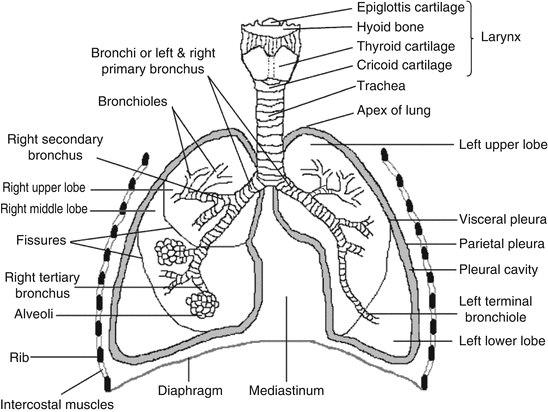
\includegraphics[scale=0.5]{9359695e86e27f8daa0bc719608a6029.png}
\end{center}
Our trachea divides into bronchi, which branch into about 20 non-symmetrical branches, which break into bronchioles, each with a diameter of about 1mm. Our bronchioles further break up into alveoli which are two thin layers of cells that separate air from blood and gasses and can freely diffuse between them. \\
The nervous system actively controls the working of the respiratory system, and its basics, like the rate of breathing, etc are controlled by the brain in the medulla region and come to the lungs through the spinal cord. The changes in metabolism are due to different types of chemical reactions in the organs of the body, which regulate the process of respiration. The sensors are basically chemo-receptors that regulate the breathing process and are directly affected by the concentration of $O_2$, $N_2$ and $CO_2$
\section{Artificial Ventilation}
In respiratory failure or insufficiency, hospitals and immediate care institutions provide artificial ventilation to provide enough oxygen and eliminate the right amount of carbon dioxide. \\The mechanical parts involved in working the ventilator are :
\begin{enumerate}
    \item Mask 
    \item Breathing valve
    \item Self-filling bag
\end{enumerate}
\begin{center}
    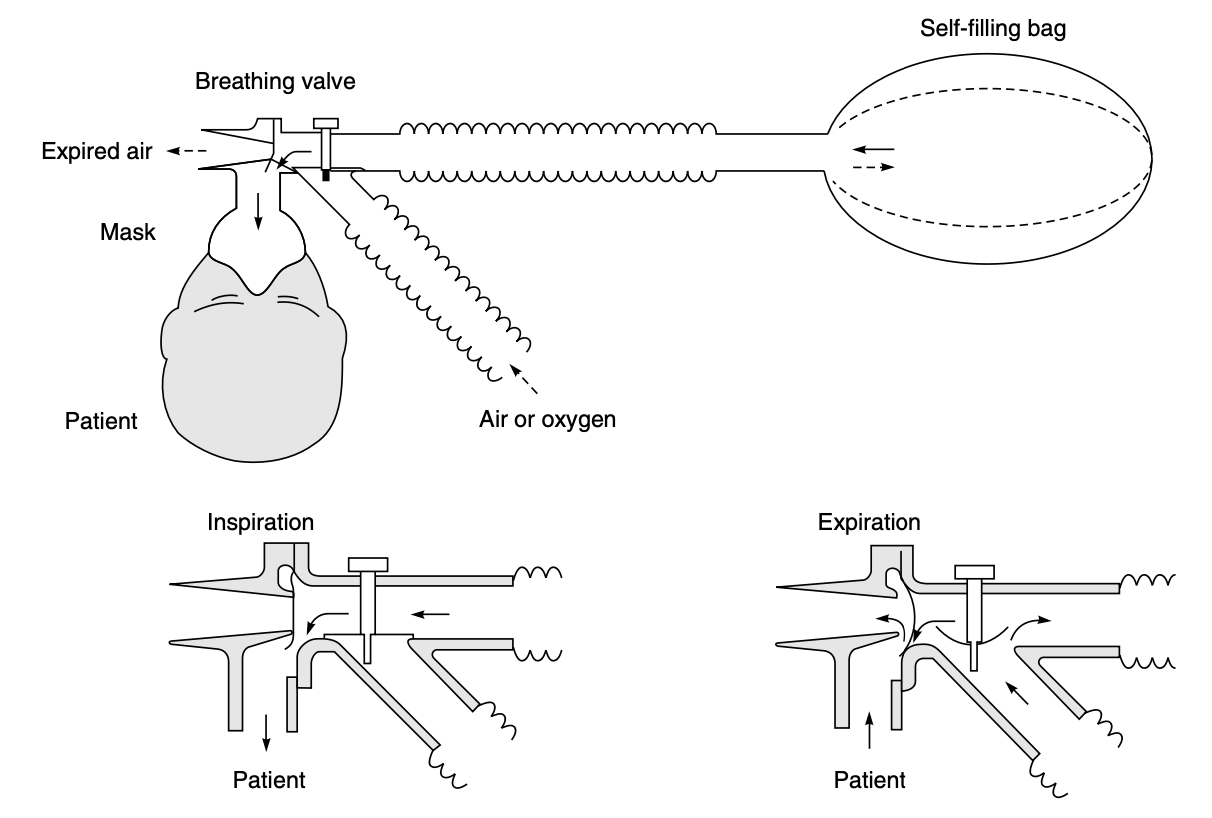
\includegraphics[scale=0.5]{Screenshot 2023-04-29 at 4.09.21 PM.png}
\end{center}
\section{Ventilators}
If artificial ventilation is to be maintained for a significant period, we employ ventilators.  They are also used when a patient is given general anaesthesia to maintain the basic human breathing pattern to sustain the patient. However, for short-term usage, resuscitators are still employed. \\\
When working with ventilators, we usually divide them into two types of pressure-controlled ventilators.
\begin{enumerate}
    \item Negative-Pressure - When a natural inspiration happens, a negative pressure is created in the pleural cavity generated by the movement of the diaphragm. In this design, the airflow to the lungs is facilitated by generating a negative pressure inside the lungs, resulting in a pressure gradient. The market did not widely accept these sorts of ventilators due to the difficulty of accessing the patient for care and monitoring.
    \item Positive-Pressure - When we generate the inspiratory flow by applying a positive pressure greater than 1 atm to the airways. These were found to be really popular, were very well received by the market, and have been responsible for treating a wide range of pulmonary disorders. It works in either mandatory or spontaneous mode. The spontaneous mode works to respond to the patient's effort the breath independently and acts as a supplemental support for respiration. They allow the patient to control the rate and volume of respiration for the patient and usually are employed for patients halfway or a certain way through their recovery. However, in the mandatory mode, the ventilator covers all the aspects of the respiratory output like tidal volume, rate of respiration and other vital elements.
\end{enumerate}
\section{Ventilator Terminology}
\begin{enumerate}
    \item Lung Compliance - It is the ratio of volume delivered to the lung to the pressure caused because of the inflow. It is usually expressed in litres/cm $H_2O$. It is the availability of the lungs to expand on inspiration.
    \begin{equation}
        Compliance = \frac{Ratio\;of\;Volume\; Delivered}{Pressure\; rise\; during\; inspiration}
    \end{equation}
    \item Airway Resistance - Ease with which air flows through the tubular respiratory structures. Resistance is inversely proportional to the diameter of the tube through which air flows.
    \item Mean Airway Pressure - An $integral$ taken over one complete cycle of pressure.
    \item Inspiratory Pause Time - The period of no flow when the pressure in the patient circuit and alveoli is the same. 
    \item Inspiratory Flow - Positive flow in the graph given below.
    \item Expiratory Flow - Negative flow in the graph given below.
    \item Tidal Volume - Depth of breathing or the volume of gas inspired or expired during each respiratory cycle.
    \begin{equation}
        Tidal\; Volume\; = Flow\;Rate\;\times\;Inspiratory\; Volume
    \end{equation}
    \item Minute Volume - This refers to volume of gas exchanged per minute of quiet breathing.
    \begin{equation}
        Minute\; Volume\; = Tidal\; Volume\; \times Breathing\; Rate
    \end{equation}
    \item Respiration Rate - The number of breaths per minute. In SIMV, The ventilator measures the previous four breaths and then shows the average total rate, which is the prescribed rate + the additional breaths taken by the patient
    \item Intermittent Mandatory Ventilation - This allows the insertion of a variable time delay between each breath.
    \item Inspiratory - Expiratory Phase time ratio - This defines the ratio of inspiratory interval to the expiratory interval of a mandatory breath. This ratio is normally limited to 1:1, but should not exceed 50\% of the total ventilation cycle.
    \item Synchronised Intermittent Mandatory Ventilation - It provides a best-of-both-world scenario where it enables the patient to breathe in spontaneously in regular breathing cycles, with the mandatory system kicking in place to support the patient during the remaining cycles. \\ 
    \begin{center}
        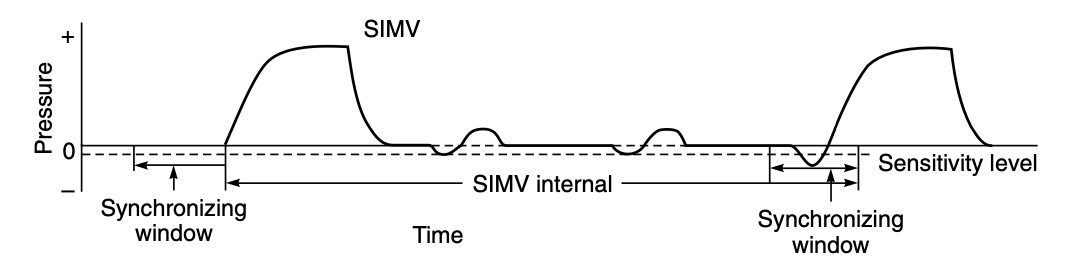
\includegraphics[scale=0.5]{Screenshot 2023-04-29 at 4.31.20 PM.png}.
    \end{center}
    \item Sigh Volume - One sigh is about 150\% of the the set tidal volume (sighs).
    \item Patient Circuit - Set of tools making the air pathway from the machine to the patient and back.
    \item Oxygen Percentage ($F_1O_2$) - In all ventilation modes, oxygen is delivered during the inspiratory phase and the percentage ($F_1O_2$) is adjustable from 21 to 91\%
    \item Peak Airway Pressure - Highest level of pressure reached over several breaths.
    \item Spontaneous Ventilation - Ventilation mode in which patient initiates and breathes from ventilator at will.
    \item Bias Flow - In Bias Flow, mixed gases from the mixer is directed through the patient circuit in-between mechanical breaths. It is there in order for the stabilisation of the baseline pressure.
    \item Sensitivity - It is put in order to sense the spontaneous effort put in by the patient in order to breathe.
    \item Mandatory Minute Volume Ventilation - This put in place if the spontaneous breathes by the patients fall below the required parameters to maintain ventilation.
    \item Controlled Mandatory Ventilation - This is referred to patients who are not able to initiate or respire on their own.
    \item Assisted Spontaneous Breathing - It refers to pressure support provided in case of insufficient spontaneous breathing by patient.
    \item Positive End Expiratory Pressure - PEEP is a doctor-selected pressure level for the patient airway at the end of expiration in either mandatory or spontaneous cycles, and is used to increase end-expiratory lung volume or prolong expiration with similar effect on the EELV.
    \item Continuous Positive Airway Pressure(CPAP) - It is a spontaneous ventilation mode in which the ventilator maintains the constant pressure to be positive, near or below the PEEP level, while the patient performs a spontaneous cycle of breathing.
    \item Assist Ventilation - It is the pressure provided to the patient in every spontaneous breathe to reach a pre-set trigger value setting. If the trigger value is not reached, it automatically moves to provide breaths at a constant pre set rate.
    \end{enumerate}
\section{Classification of Ventilators}
\subsection{Basis of initiating respiratory flow}
\begin{enumerate}
    \item Controller - It works independent of the patients efforts and will to breathe and is mostly employed to patients who are unable to breathe on their at all.
    \item Assistor - It is an augmentation factor in the inspiration of the patient by operating in response to the patient's inspiration efforts. A piezo sensor detects the negative pressure induced every time the patients attempts to inhale and then it triggers the process of inflating the lungs. It has a sensitivity adjustment provided on the equipment which helps us to select the amount of pressure required on the part of the patient.
    \item Assistor/Controller - A ventilator which works on the amalgamation of the workings of both the types of ventilators, where it assists the patient to breathe but in case the patient fails to breathe within a pre determined time the machine takes over and continues to trigger inspiration of the lungs for a pre-determined time. It is mostly employed in CCU.
\end{enumerate}
\subsection{Based on Power Transmission}
\begin{enumerate}
    \item Direct Power Transmission - Delivers gas directly from the source of compressed gas to the patient
    \item Indirect Power Transmission - Separated power and patient systems. The pressure in power system here determines flow rate.
\end{enumerate}
\subsection{Based on Pressure Pattern}
\begin{enumerate}
    \item Positive - Atmosphere - Here the end expiratory pressure is adjusted to be the same as the atmospheric pressure. In this the mode, the patient breathes spontaneously.
    \item Positive - Negative - Here the end-expiratory pressure is less than the atmospheric pressure.
    \item Positive - Positive - The end expiratory pressure is greater than the atmospheric pressure.
\end{enumerate}
\subsection{Based on Safety limit}
\begin{enumerate}
    \item Volume Limited - Tidal Volume being the limit.
    \item Pressure Limited
    \item Time Limited
\end{enumerate}
\subsection{Based on Cycling Control}
\subsubsection{Cycling from inspiration to expiration}
\begin{enumerate}
    \item Volume Cycled - Target to achieve a preset Tidal Volume, then initiate expiration phase.
    \item Pressure Cycled - Target to attain a preset pressure, then initiate expiration phase.
    \item Time Cycled - Starts expiration after a certain present time period of inspiration has expired.
\end{enumerate}
\subsubsection{Cycling from expiration to inspiration}
\begin{enumerate}
    \item Pressure Cycled - Begins inspiration, after a preset expiratory pressure has been established.
    \item Time Cycled - A ventilator which initiates the inspiratory phase after present time period of expiration expires.
    \item Patient Inspiratory Effort Cycled - Starts as an effect to patients inspiratory efforts. 
\end{enumerate}
\subsection{Based on Source of Power}
\begin{enumerate}
    \item Pneumatic 
    \item Electric
\end{enumerate}
\section{Analysis of Pressure, flow and volume diagrams}
\begin{center}
    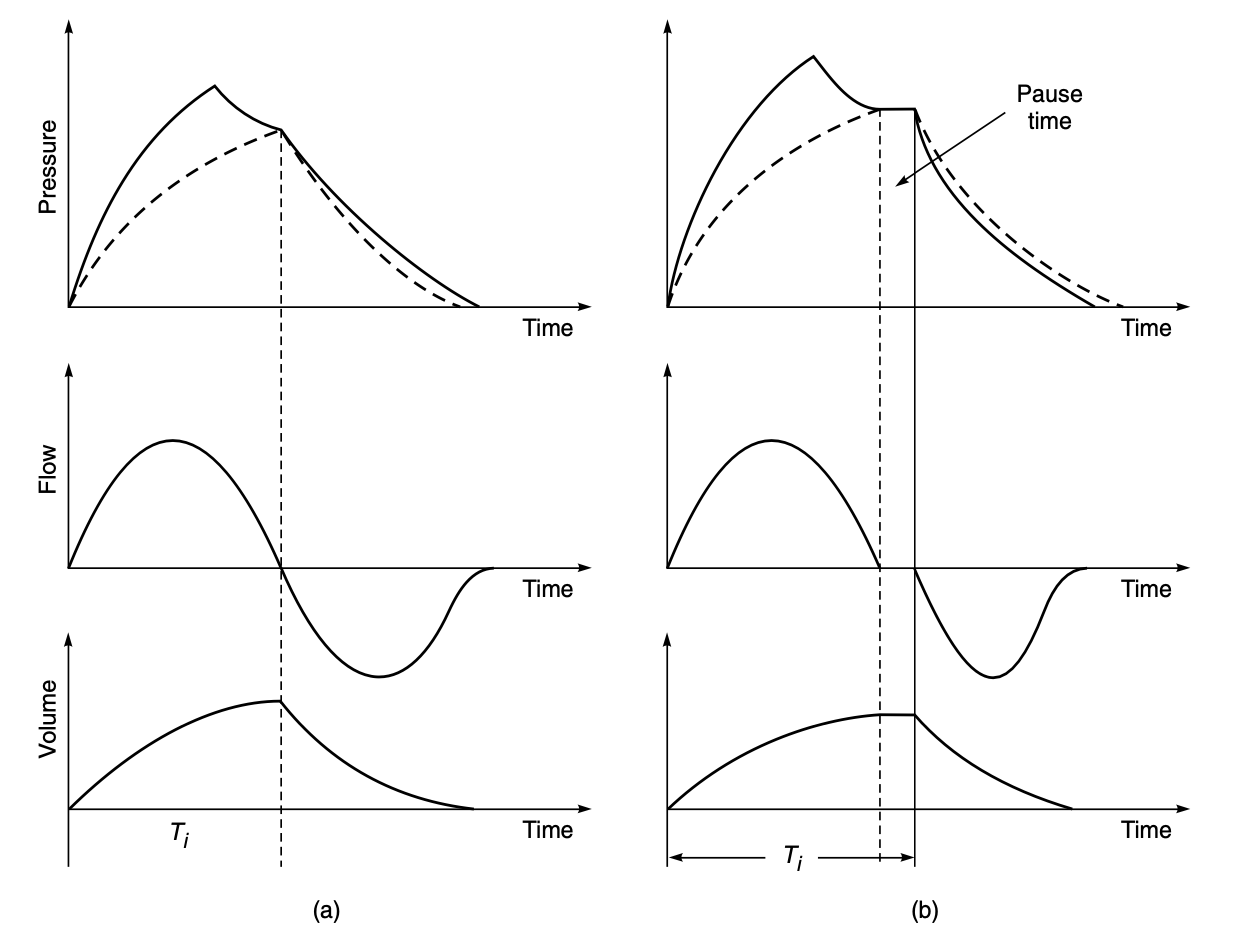
\includegraphics[scale = 0.5]{Graphs.png}
\end{center}
\section{Requirements and basics needed in a modern day ventilator}
With the expanse of technology and the way the medical industry works now, any basic ventilation device even should have the qualities to provide precise flow, pressure and oxygen control with negligible time lag, patient monitoring and an emergency alert system for patient mishaps.\\\\
The design of any modern day ventilator should have a clear distinction between pneumatic and the electrical system and should have the capacity to coordinate between the two without any issues.\\
\newpage
\begin{center}
    \textbf{Block Diagram of a modern Ventilator}\\
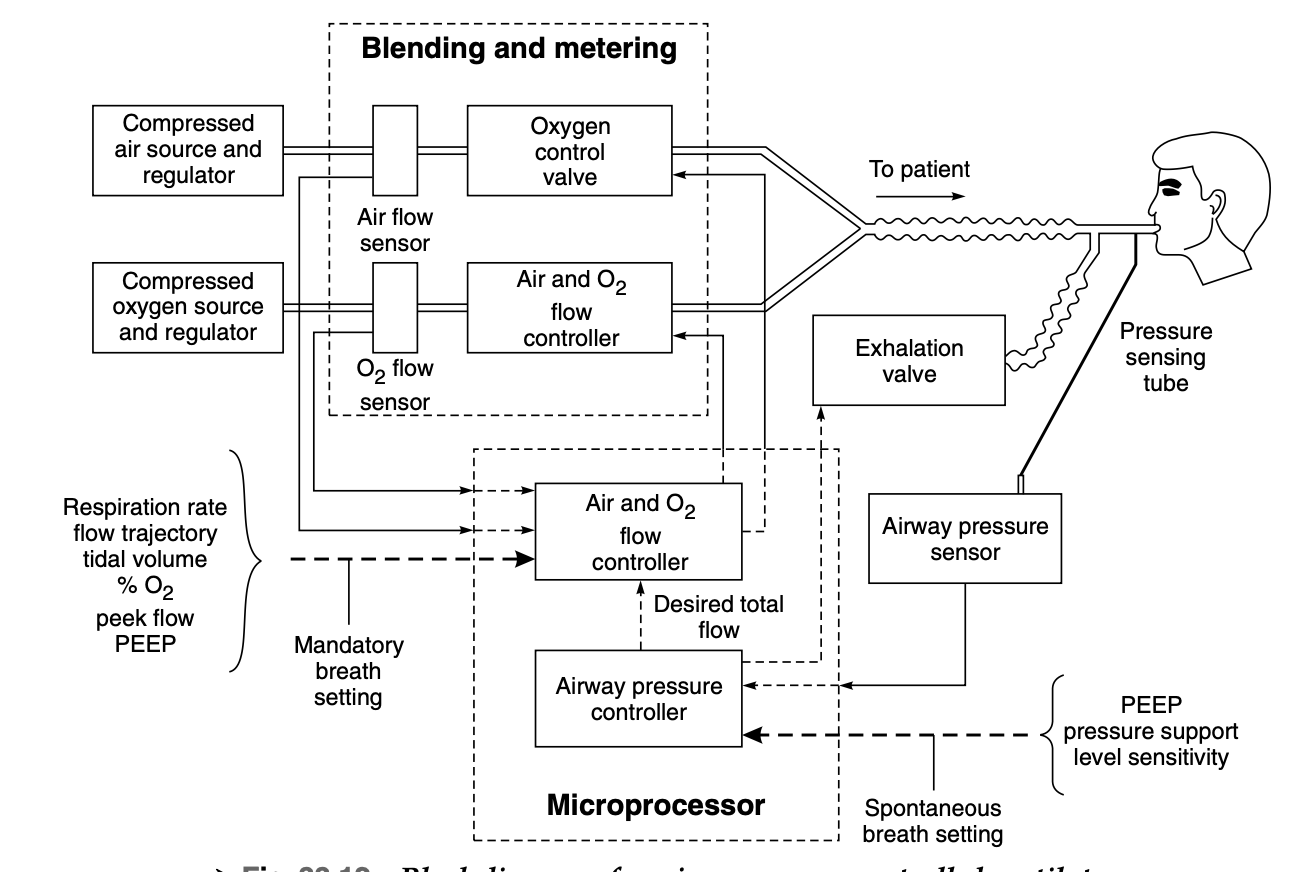
\includegraphics[scale = 0.5]{BlockDiagram.png}\\
\end{center}
\section{High Frequency Ventilators}
In recent studies, ventilation of patients at a rate much higher than the respiration rate has been recently introduced and has shown records of improved levels of $CO_2$ wash out than average ventilators, and also have shown a better quality of oxygenation. \textbf{The key principle of working of the HFV is providing Tidal Volume equal to or smaller than the dead space at very high rates.}

\end{document}
